\section{Results}\label{sec:results}
In this section, we present the findings from the thorough tests that were discussed in the previous section. The significant amount of time needed for the code to run across various aggregation systems is the main obstacle for carrying out these tests, as was previously mentioned. To ensure extensive evaluations of the proposed strategies' effectiveness, a substantial amount of time is required.

Additionally, as discussed in the previous section, our main goal is to optimise the ASR, while also maintaining an acceptable value of overall accuracy.

This guarantees that our attack only affects the targeted classes while maintaining a reasonable performance across the full range of classifications. The upcoming findings shed light on the performance of the hypotheses discussed in Sections \ref{sec:entropy_label_flipping}, \ref{sec:closeness_label_flipping}, and \ref{sec:adaptive_label_flipping}.

We will also comment the results obtained from the experiments that were carried out to evaluate the effectiveness of the strategies for the MNIST dataset.
%%%%%%%%%%%%%%%%%%%%%%%%%%%%%%%%%%%%%%%%%%%%%%%%%%%%%%%%%%%%%%%
\subsection{Results for the MNIST dataset}
The experiments for this dataset were carried out using the following values for the specified parameters:
\begin{itemize}
        \item The data distribution type was changed from non-IID to IID.
        \item The number of peers was changed from 100 to 50.
        \item the amount of global rounds was changed from 200 to 50.
\end{itemize}

The first step is to evaluate which are the results for the baseline model\footnote{The baseline model is the model that is trained without any attack.}. The baseline for a FL setting is FedAvg, since it is the aggregation method specified in the proposal of this system \cite{FederatedLearningPaper}. We also evaluate the performance for the standard label flipping attack to be able to compare it with the proposed strategies.

\subsubsection{MNIST results with an attacker's ratio of 10\%}
The first experiment is performed for the standard label flipping attack. The results are shown in \autoref{tab:standard_mnist_10}. 
As it can be seen, we do not perform all the possible experiments, since at this point of the project we are interested in evaluating the performance of our hypotheses with the specified attacker's ratio. For future reference, \autoref{fig:confusion_reference} shows the confusion matrix for the baseline model, where there have been no attacks and the model is almost perfectly trained.
\begin{table}[h]
        \centering
        \begin{tabular}{|c|c|c|c|c|c|}
            \hline
            & FedAvg (No Attackers) & FedAvg & Median & TMean & MKrum\\
            \hline
            TE & 0.0519 & 0.055 & 0.055 & 0.0539 & 0.0522 \\
            \hline
            All-Acc & 98.35 & 98.34 & 98.36 & 98.36 & 98.41 \\
            \hline
            Src-Acc & 97.28 & 96.4 & 96.89 & 96.98 & 97.67 \\
            \hline
            ASR & 0.29 & 0.39 & 0.29 & 0.29 & 0.29 \\
            \hline
        \end{tabular}
        \caption{MNIST. Standard label flipping, attacker's ratio of 10\%}
        \label{tab:standard_mnist_10}
\end{table}

\begin{figure}[h!]
        \centering
        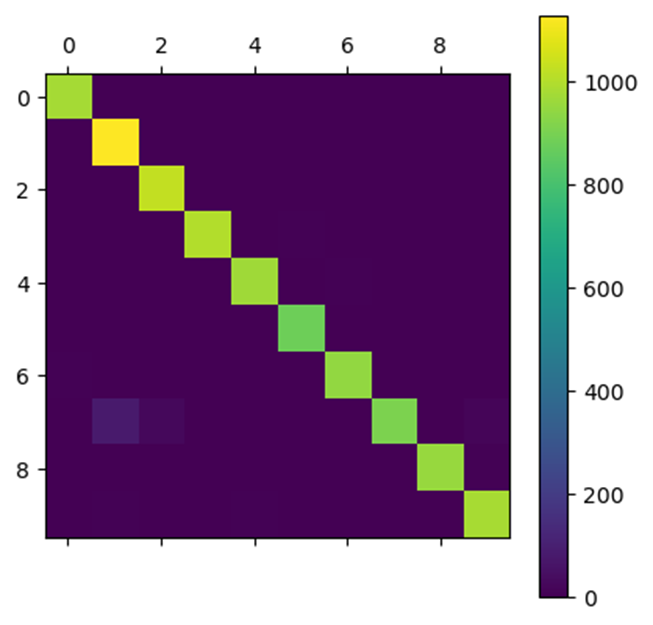
\includegraphics[scale=0.88]{confusion_reference.png}
        \caption{Confusion matrix for the baseline model}
        \label{fig:confusion_reference}
\end{figure}

\autoref{tab:entropy_mnist_10_top_25} shows the results obtained when testing the top 25\% entropy and an attacker's ratio of 10\%.
The obtained results are similar to the results for the standard label flipping attack, except for FedAvg, where the ASR drops by 0.20\%.
\begin{table}[h!]
        \centering
        \begin{tabular}{|c|c|c|c|c|}
            \hline
            & FedAvg & Median & TMean & MKrum \\
            \hline
            TE & 0.0509 & 0.0546 & 0.0539 & 0.0516 \\
            \hline
            All-Acc & 98.42 & 98.31 & 98.36 & 98.38 \\
            \hline
            Src-Acc & 97.57 & 97.47 & 97.47 & 97.57 \\
            \hline
            ASR & 0.19 & 0.29 & 0.29 & 0.29 \\
            \hline
        \end{tabular}
        \caption{MNIST. Entropy-based label flipping, top 25\% entropy, attacker's ratio of 10\%}
        \label{tab:entropy_mnist_10_top_25}
    \end{table}

\subsubsection{MNIST results with an attacker's ratio of 40\%}

Since the results for an attacker's ratio of 10\% are not very promising, we decided to increase the attacker's ratio to 40\% to see if the results improve.
\autoref{tab:standard_mnist_40} shows the results obtained for the standard label flipping attack and an attacker's ratio of 40\%. Note that for this experiment, the baseline is not tested, and only two aggregation methods are evaluated.
As seen in the table, the ASR improves for both aggregation methods.
\begin{table}[h!]
        \centering
        \begin{tabular}{|c|c|c|}
            \hline
            & FedAvg & TMean \\
            \hline
            TE & 0.0985 & 0.0653 \\
            \hline
            All-Acc & 97.56 & 98.11 \\
            \hline
            Src-Acc & 87.94 & 94.55 \\
            \hline
            ASR & 7.78 & 1.46 \\
            \hline
        \end{tabular}
        \caption{MNIST. Standard label flipping, attacker's ratio of 40\%}
        \label{tab:standard_mnist_40}
    \end{table}
    
Finally, \autoref{tab:entropy_mnist_40_top_25} shows the results obtained for the entropy-based label flipping attack and an attacker's ratio of 40\%.
The results are not promising when compared to the results for the standard label flipping attack.

\begin{table}[h!]
        \centering
        \begin{tabular}{|c|c|c|}
            \hline
            & FedAvg & TMean \\
            \hline
            TE & 0.0533 & 0.0556 \\
            \hline
            All-Acc & 98.46 & 98.38 \\
            \hline
            Src-Acc & 97.57 & 97.57 \\
            \hline
            ASR & 0.19 & 0.19 \\
            \hline
        \end{tabular}
        \caption{MNIST. Entropy-based label flipping, top 25\% entropy, attacker's ratio of 40\%}
        \label{tab:entropy_mnist_40_top_25}
    \end{table}
We first began using the MNIST dataset for our experiments because it is the most common dataset used in the literature. However, we quickly realized that the results were not very interesting. The reason for this is that the MNIST dataset is too simple. The model is able to achieve a very high accuracy, and the label flipping attacks are not able to reduce it significantly. Therefore, we decided to use the CIFAR-10 dataset instead. This dataset is more complex, and the model is not able to achieve such a high accuracy. This means that the label flipping attacks are able to reduce the accuracy significantly. In the following sections, we present the results obtained with the MNIST dataset along with the ones obtained with the CIFAR-10 dataset. The reason behind this is to show the difference between both datasets. However, we focus on the results obtained with the CIFAR-10 dataset because they are more interesting. Our aim will be to flip the labels of the source class (dog) to the target class label (cat). 
    

\subsection{Results for the CIFAR-10 dataset}
Since the results obtained with the MNIST dataset are not promising, we decided to evaluate the performance of the proposed strategies with the CIFAR-10 dataset.
MNIST offers a relatively easy problem to solve, since the images are very simple. This is why the aggregation methods are able to achieve a very high accuracy.

The aim for these experiments is finding which attack obtains the best results in order to evaluate the performance of the proposed strategies on lower attacker's ratio. This is why, for some strategies' modifications, we only evaluate the performance for some aggregation methods.

%%%%%%%%%%%%%%%%%%%%%%%%%%%%%%%%%%%%%%%%%%%%%%%%%%%%%%%%%%%%%%%
\subsubsection{CIFAR-10 results with an attacker's ratio of 30\%}\label{sec:cifar_30}
We begin these experiments with an attacker's ratio of 30\%, using the parameters commented in \ref{sec:chosen_parameters}.
\autoref{tab:standard_cifar_30} shows the results obtained for the standard label flipping attack.
As it can be seen, the ASR is very high for almost all the aggregation methods, this way it will be easier to detect if the proposed strategies are effective.

\begin{table}[h!]
        \centering
        \small
        \begin{adjustbox}{center}
        \begin{tabular}{|c|c|c|c|c|c|c|c|c|c|}
            \hline
            & FedAvg (NA) & FedAvg & Median & TMean & MKrum & Foolsgold & Tolpegin & FLAME & LFighter \\
            \hline
            TE & 0.8058 & 0.8935 & 0.8462 & 0.872 & 1.0101 & 0.8821 & 0.9063 & 1.1157 & 0.8891 \\
            \hline
            All-Acc & 76.56 & 75.02 & 74.8 & 75.35 & 72.7 & 75.85 & 74.77 & 72.97 & 74.8 \\
            \hline
            Src-Acc & 65.6 & 35.4 & 36.0 & 35.0 & 17.5 & 63.9 & 60.4 & 21.3 & 62.2 \\
            \hline
            ASR & 14.7 & 43.2 & 41.6 & 45.3 & 62.7 & 15.8 & 15.4 & 55.5 & 15.2 \\
            \hline
        \end{tabular}
        \end{adjustbox}
        \caption{Standard label flipping, attacker's ratio of 30\%}
        \label{tab:standard_cifar_30}
\end{table}

The results for the entropy-based label flipping attack, which flips the 25\% highest entropies are shown in \autoref{tab:entropy_cifar_30_top_25}.
As it can be seen, the ASR is lower than the ASR obtained for the standard label flipping attack. The next step is to increment the amount of labels flipped to see if the results improve.

\begin{table}[h!]
        \centering
        \small
        \begin{adjustbox}{center}
        \begin{tabular}{|c|c|c|c|c|c|c|c|c|}
            \hline
            & FedAvg & Median & TMean & MKrum & Foolsgold & Tolpegin & FLAME & LFighter \\
            \hline
            TE & 0.8074 & 0.7735 & 0.7821 & 0.8867 & 0.8059 & 0.8379 & 0.9565 & 0.8709 \\
            \hline
            All-Acc & 76.7 & 76.4 & 76.37 & 76.45 & 76.72 & 76.39 & 76.24 & 76.85 \\
            \hline
            Src-Acc & 61.2 & 61.7 & 61.2 & 58.3 & 60.2 & 59.8 & 58.8 & 61.8 \\
            \hline
            ASR & 17.4 & 18.5 & 18.7 & 20.7 & 19.5 & 19.4 & 19.8 & 17.7 \\
            \hline
        \end{tabular}
        \end{adjustbox}
        \caption{Entropy-based label flipping, top 25\% entropy, attacker's ratio of 30\%}
        \label{tab:entropy_cifar_30_top_25}
    \end{table}
    
\autoref{tab:entropy_cifar_30_top_50} shows the results obtained for the entropy-based label flipping attack, which flips the 50\% highest entropies.
This attack is the one selected to represent entropy in experiments with lower attacker's ratio, since it obtains good results without incrementing too much the amount of labels flipped.

\begin{table}[h!]
        \centering
        \small
        \begin{adjustbox}{center}
        \begin{tabular}{|c|c|c|c|c|c|c|c|c|}
            \hline
            & FedAvg & Median & TMean & MKrum & Foolsgold & Tolpegin & FLAME & LFighter \\
            \hline
            TE & 0.8301 & 0.8092 & 0.8146 & 0.8978 & 0.8402 & 0.8421 & 1.0441 & 0.8724 \\
            \hline
            All-Acc & 76.38 & 75.48 & 75.55 & 75.4 & 76.62 & 76.38 & 73.88 & 76.13 \\
            \hline
            Src-Acc & 56.3 & 54.6 & 54.5 & 51.2 & 55.1 & 53.5 & 46.9 & 62.6 \\
            \hline
            ASR & 22.3 & 25.3 & 24.1 & 25.7 & 23.0 & 25.8 & 26.5 & 15.6 \\
            \hline
        \end{tabular}
        \end{adjustbox}
        \caption{Entropy-based label flipping, top 50\% entropy, attacker's ratio of 30\%}
        \label{tab:entropy_cifar_30_top_50}
    \end{table}
    

The results for the entropy-based label flipping attack, which flips the 75\% highest entropies are shown in \autoref{tab:entropy_cifar_30_top_75}. We can observe higher results when compared with the strategy flipping 50\% of the samples. Given that the results do not improve by a huge factor, we will not use this strategy in the experiments with lower attacker's ratio since the amount of extra labels flipped is considered to be too high.

\begin{table}[h!]
        \centering
        \small
        \begin{adjustbox}{center}
        \begin{tabular}{|c|c|c|}
            \hline
            & FedAvg & TMean \\
            \hline
            TE & 0.8353 & 0.8277 \\
            \hline
            All-Acc & 76.08 & 75.59 \\
            \hline
            Src-Acc & 48.6 & 47.3 \\
            \hline
            ASR & 29.1 & 28.3 \\
            \hline
        \end{tabular}
        \end{adjustbox}
        \caption{Entropy-based label flipping, top 75\% entropy, attacker's ratio of 30\%}
        \label{tab:entropy_cifar_30_top_75}
    \end{table}

\autoref{tab:entropy_cifar_30_low_50} shows the results obtained for the entropy-based label flipping attack, which flips the 50\% lowest entropies. The results are close to those obtained when flipping the highest 50\% entropies, but the ASR is lower while flipping the same amount of labels.


\begin{table}[h!]
        \centering
        \small
        \begin{adjustbox}{center}
        \begin{tabular}{|c|c|c|c|c|c|c|c|c|}
            \hline
            & FedAvg & Median & TMean & MKrum & Foolsgold & Tolpegin & FLAME & LFighter \\
            \hline
            TE & 0.8273 & 0.8166 & 0.8263 & 0.907 & 0.8453 & 0.826 & 1.0302 & 0.8851 \\
            \hline
            All-Acc & 76.55 & 75.46 & 75.82 & 75.67 & 76.32 & 76.08 & 74.37 & 75.44 \\
            \hline
            Src-Acc & 55.4 & 54.8 & 57.8 & 53.7 & 57.0 & 56.5 & 51.9 & 61.6 \\
            \hline
            ASR & 22.9 & 23.4 & 22.1 & 25.6 & 21.0 & 22.9 & 25.1 & 16.3 \\
            \hline
        \end{tabular}
        \end{adjustbox}
        \caption{Entropy-based label flipping, lowest 50\% entropy, attacker's ratio of 30\%}
        \label{tab:entropy_cifar_30_low_50}
    \end{table}
    

The results for the entropy-based label flipping attack, which flips the 25\% lowest entropies are shown in \autoref{tab:entropy_cifar_30_low_25}. As the table shows, the ASR is lower than the ASR obtained for the strategy flipping the 50\% lowest entropies.

\begin{table}[h!]
        \centering
        \small
        \begin{adjustbox}{center}
        \begin{tabular}{|c|c|c|c|c|c|c|c|c|}
            \hline
            & FedAvg & Median & TMean & MKrum & Foolsgold & Tolpegin & FLAME & LFighter \\
            \hline
            TE & 0.824 & 0.7864 & 0.7639 & 0.8805 & 0.8068 & 0.8118 & 1.0406 & 0.902 \\
            \hline
            All-Acc & 76.7 & 76.51 & 76.88 & 76.65 & 77.07 & 76.54 & 74.8 & 76.42 \\
            \hline
            Src-Acc & 60.1 & 58.8 & 62.4 & 60.1 & 61.2 & 61.3 & 57.7 & 58.4 \\
            \hline
            ASR & 18.8 & 19.9 & 16.9 & 18.1 & 18.7 & 18.6 & 18.4 & 18.3 \\
            \hline
        \end{tabular}
        \end{adjustbox}
        \caption{Entropy-based label flipping, lowest 25\% entropy, attacker's ratio of 30\%}
        \label{tab:entropy_cifar_30_low_25}
    \end{table}

The results for an entropy-based label flipping attack, keeping the 50\% highest entropies, and boosted with a scaling factor of 1.2 are shown in \autoref{tab:entropy_cifar_30_top_50_boosted_1_2}.
As can be seen, the scaling factor either improves or lowers the ASR, depending on the aggregation method. 
The scaling factor also affects the overall accuracy, since we are scaling all weights instead of only the weights of the targeted classes. \autoref{fig:confusion_scaling1-2_foolsgold} shows the confusion matrix for FoolsGold when applying a scaling factor of 1.2. As can be seen, the overall accuracy is lowered. In this case, the effect is that most classes are classified as class 4, which is not the source nor the target class.
\begin{table}[h!]
        \centering
        \small
        \begin{adjustbox}{center}
        \begin{tabular}{|c|c|c|c|c|c|c|c|c|}
            \hline
            & FedAvg & Median & TMean & MKrum & Foolsgold & Tolpegin & FLAME & LFighter \\
            \hline
            TE & 1.7627 & 1.2765 & 1.3963 & 0.9382 & 1.7487 & 0.8719 & 1.1691 & 0.872 \\
            \hline
            All-Acc & 36.02 & 54.27 & 49.37 & 74.87 & 38.21 & 76.65 & 73.39 & 76.28 \\
            \hline
            Src-Acc & 28.5 & 36.4 & 10.0 & 64.0 & 33.9 & 64.3 & 62.1 & 64.4 \\
            \hline
            ASR & 14.0 & 44.9 & 73.9 & 16.2 & 16.7 & 14.6 & 16.5 & 14.4 \\
            \hline
        \end{tabular}
        \end{adjustbox}
        \caption{Entropy-based label flipping, top 50\% entropy, scaling factor of 1.2, attacker's ratio of 30\%}
        \label{tab:entropy_cifar_30_top_50_boosted_1_2}
    \end{table}
    

\begin{figure}[h!]
        \centering
        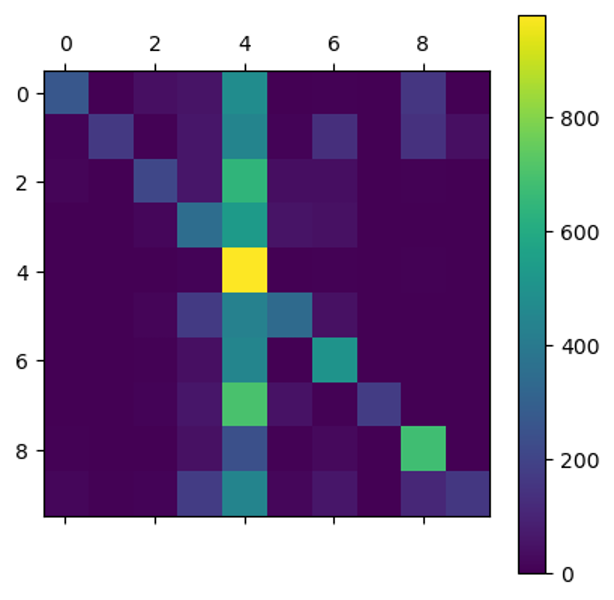
\includegraphics[scale=0.88]{confusion_scaling1-2_foolsgold.png}
        \caption{Confusion matrix for FoolsGold when applying a scaling factor of 1.2}
        \label{fig:confusion_scaling1-2_foolsgold}
\end{figure}

\autoref{tab:entropy_cifar_30_top_50_boosted_1_1} shows the results obtained for the entropy-based label flipping attack, which flips the 50\% highest entropies, and boosted with a scaling factor of 1.1. From these results we can extract that modifying the scaling factor while flipping the top 50\% entropy samples is not improving the results. Our next step is to try applying a scaling factor after flipping the highest 25\% entropy samples.

\begin{table}[h!]
        \centering
        \small
        \begin{adjustbox}{center}
        \begin{tabular}{|c|c|c|c|c|c|c|c|c|}
            \hline
            & FedAvg & Median & TMean & MKrum & Foolsgold & Tolpegin & FLAME & LFighter \\
            \hline
            TE & 2.1662 & 1.2913 & 1.4383 & 0.9225 & 2.101 & 0.8495 & 1.0811 & 0.8697 \\
            \hline
            All-Acc & 21.26 & 52.55 & 47.58 & 74.61 & 23.59 & 76.88 & 73.46 & 75.3 \\
            \hline
            Src-Acc & 9.6 & 24.3 & 13.9 & 64.8 & 18.7 & 64.4 & 61.7 & 61.4 \\
            \hline
            ASR & 15.1 & 56.2 & 63.5 & 15.0 & 17.5 & 14.4 & 16.3 & 16.6 \\
            \hline
        \end{tabular}
        \end{adjustbox}
        \caption{Entropy-based label flipping, top 50\% entropy, scaling factor of 1.1, attacker's ratio of 30\%}
        \label{tab:entropy_cifar_30_top_50_boosted_1_1}
    \end{table}
    
The final experiment with scaling factors is using again a factor of 1.1 and changing the entropy method to flip the top 25\% highest entropies. The results are shown in \autoref{tab:entropy_cifar_30_top_25_boosted_1_1}.
Since applying a scaling factor does not improve the results, we will not use it in the experiments with lower attacker's ratio.
\begin{table}[h!]
        \centering
        \small
        \begin{adjustbox}{center}
        \begin{tabular}{|c|c|c|c|c|c|c|c|c|}
            \hline
            & FedAvg & Median & TMean & MKrum & Foolsgold & Tolpegin & FLAME & LFighter \\
            \hline
            TE & 2.1276 & 1.3397 & 1.3826 & 0.941 & 2.1069 & 0.8886 & 1.1464 & 0.8919 \\
            \hline
            All-Acc & 23.79 & 52.91 & 50.76 & 75.55 & 23.18 & 75.5 & 73.11 & 76.37 \\
            \hline
            Src-Acc & 14.0 & 40.0 & 32.4 & 63.2 & 14.3 & 63.5 & 62.9 & 62.0 \\
            \hline
            ASR & 12.8 & 40.7 & 46.4 & 14.3 & 14.6 & 14.9 & 15.3 & 15.9 \\
            \hline
        \end{tabular}
        \end{adjustbox}
        \caption{Entropy-based label flipping, top 25\% entropy, scaling factor of 1.1, attacker's ratio of 30\%}
        \label{tab:entropy_cifar_30_top_25_boosted_1_1}
    \end{table}
    

With the experiments of the entropy-based label flipping concluded for an attacker's ratio of 30\%, we proceed to perform the proposed experiments for the closeness-based label flipping attack.

We begin by testing the closeness-based label flipping attack, which flips the 25\% closest images. The results are shown in \autoref{tab:closeness_cifar_30_top_25}. Knowing that for entropy the results improved when flipping the 50\% highest entropy samples, we test only two aggregation methods for a closeness attack where we flip the 25\% highest closeness'. This is because the amount of time taken to test the whole set of aggregation methods is very high and, if it is not a promising attack, that time can be used to test other attacks.

\begin{table}[h!]
        \centering
        \small
        \begin{adjustbox}{center}
        \begin{tabular}{|c|c|c|}
            \hline
            & FedAvg & TMean \\
            \hline
            TE & 0.8299 & 0.8235 \\
            \hline
            All-Acc & 76.63 & 76.48 \\
            \hline
            Src-Acc & 60.4 & 59.5 \\
            \hline
            ASR & 18.2 & 20.1 \\
            \hline
        \end{tabular}
        \end{adjustbox}
        \caption{Closeness-based label flipping, top 25\% closest images, attacker's ratio of 30\%}
        \label{tab:closeness_cifar_30_top_25}
    \end{table}


\autoref{tab:closeness_cifar_30_top_50} shows the results obtained for the closeness-based label flipping attack, which flips the 50\% closest images. This attack is the one selected to represent closeness in experiments with lower attacker's ratio, since it obtains good results without incrementing too much the number of labels flipped. As can be seen, we have taken a good choice not testing all the aggregation methods for the 25\% closest images.

\begin{table}[h!]
        \centering
        \small
        \begin{adjustbox}{center}
        \begin{tabular}{|c|c|c|c|c|c|c|c|c|}
            \hline
            & FedAvg & Median & TMean & MKrum & Foolsgold & Tolpegin & FLAME & LFighter \\
            \hline
            TE & 0.8205 & 0.8455 & 0.806 & 0.9058 & 0.8301 & 0.8467 & 1.0287 & 0.9029 \\
            \hline
            All-Acc & 76.23 & 76.68 & 76.08 & 75.83 & 76.7 & 76.47 & 74.24 & 75.05 \\
            \hline
            Src-Acc & 52.0 & 55.4 & 53.2 & 47.9 & 54.0 & 55.6 & 43.8 & 64.0 \\
            \hline
            ASR & 26.3 & 23.6 & 25.7 & 31.8 & 23.6 & 23.2 & 32.9 & 13.8 \\
            \hline
        \end{tabular}
        \end{adjustbox}
        \caption{Closeness-based label flipping, top 50\% closest images, attacker's ratio of 30\%}
        \label{tab:closeness_cifar_30_top_50}
    \end{table}
    


To conclude with the closeness-based label flipping, we perform the experiments for different thresholds. \autoref{tab:closeness_cifar_30_threshold_0-3} shows the results obtained for the closeness-based label flipping attack, which flips the samples that have a closeness value lower than 0.3. The rationale behind not testing all the aggregation methods is the same as the one explained for the closeness-based label flipping attack that flips the 25\% closest images.

\begin{table}[h!]
        \centering
        \small
        \begin{adjustbox}{center}
        \begin{tabular}{|c|c|c|}
            \hline
            & FedAvg & TMean \\
            \hline
            TE & 0.82 & 0.7903 \\
            \hline
            All-Acc & 76.56 & 76.5 \\
            \hline
            Src-Acc & 63.0 & 65.5 \\
            \hline
            ASR & 15.9 & 14.8 \\
            \hline
        \end{tabular}
        \end{adjustbox}
        \caption{Closeness-based label flipping, threshold of 0.3, attacker's ratio of 30\%}
        \label{tab:closeness_cifar_30_threshold_0-3}
    \end{table}
    
The results for a threshold of 0.6 are shown in \autoref{tab:closeness_cifar_30_threshold_0-6}. As can be seen, the results improve by using a higher threshold. However, flipping samples with a closeness value lower than 0.6 is not a good strategy, since the ASR is lower than the ASR obtained for the strategy flipping the 50\% closest images.


\begin{table}[h!]
        \centering
        \small
        \begin{adjustbox}{center}
        \begin{tabular}{|c|c|c|}
            \hline
            & FedAvg & TMean \\
            \hline
            TE & 0.825 & 0.7901 \\
            \hline
            All-Acc & 76.67 & 76.52 \\
            \hline
            Src-Acc & 64.4 & 64.6 \\
            \hline
            ASR & 15.8 & 16.1 \\
            \hline
        \end{tabular}
        \end{adjustbox}
        \caption{Closeness-based label flipping, threshold of 0.6, attacker's ratio of 30\%}
        \label{tab:closeness_cifar_30_threshold_0-6}
    \end{table}

Since the experiments carried out using a threshold do not improve the results, we will not use this strategy in the experiments with lower attacker's ratio.

The final experiments for an attacker's ratio of 30\% are performed with the adaptive label flipping attack, using entropy. The first tested strategy is the one that flips the 100\% of the samples during the first 25 rounds, 75\% during the rounds in the range of 25-50, 50\% during the rounds in the range of 50-75, and 25\% during the last 25 rounds. The results are shown in \autoref{tab:adaptive_cifar_30_100_75_50_25}. The obtained results are not promising when compared to the results obtained for the entropy or closeness-based label flipping attacks.

\begin{table}[h!]
        \centering
        \small
        \begin{adjustbox}{center}
        \begin{tabular}{|c|c|c|c|c|c|c|c|c|}
            \hline
            & FedAvg & Median & TMean & MKrum & Foolsgold & Tolpegin & FLAME & LFighter \\
            \hline
            TE & 0.8327 & 0.787 & 0.8044 & 0.8875 & 0.8272 & 0.8427 & 1.0105 & 0.8576 \\
            \hline
            All-Acc & 76.56 & 76.93 & 76.44 & 76.46 & 76.33 & 76.45 & 74.17 & 75.95 \\
            \hline
            Src-Acc & 59.2 & 63.1 & 60.9 & 58.4 & 59.1 & 61.4 & 54.1 & 58.7 \\
            \hline
            ASR & 19.5 & 18.2 & 18.6 & 20.1 & 19.8 & 18.6 & 23.7 & 19.1 \\
            \hline
        \end{tabular}
        \end{adjustbox}
        \caption{Adaptive label flipping (entropy), 100 75 50 25, attacker's ratio of 30\%}
        \label{tab:adaptive_cifar_30_100_75_50_25}
    \end{table}
    
\autoref{tab:adaptive_cifar_30_100_50} shows the results obtained for the adaptive label flipping attack, which flips the 100\% of the samples during the first 50 rounds, and the 50\% samples with highest entropy during the last 50 rounds. The results are better than those obtained for the entropy and closeness-based label flipping attacks, but following the rationale of the top 75\% entropies, we will not use this strategy in the experiments with lower attacker's ratio since the amount of extra labels flipped is considered to be too high.

\begin{table}[h!]
        \centering
        \small
        \begin{adjustbox}{center}
        \begin{tabular}{|c|c|c|c|c|c|c|c|c|}
            \hline
            & FedAvg & Median & TMean & MKrum & Foolsgold & Tolpegin & FLAME & LFighter \\
            \hline
            TE & 0.825 & 0.7872 & 0.8134 & 0.8913 & 0.8538 & 0.8856 & 1.0319 & 0.8958 \\
            \hline
            All-Acc & 76.08 & 76.41 & 76.08 & 75.95 & 76.15 & 75.85 & 75.69 & 74.92 \\
            \hline
            Src-Acc & 55.0 & 55.3 & 55.3 & 53.6 & 63.2 & 51.6 & 51.5 & 63.0 \\
            \hline
            ASR & 23.4 & 22.9 & 23.4 & 26.3 & 15.7 & 26.3 & 27.6 & 15.9 \\
            \hline
        \end{tabular}
        \end{adjustbox}
        \caption{Adaptive label flipping (entropy), 100 50, attacker's ratio of 30\%}
        \label{tab:adaptive_cifar_30_100_50}
    \end{table}
    
The results for the adaptive label flipping attack, which flips the 100\% of the samples during the first 50 rounds, and the 25\% samples with highest entropy during the last 50 rounds are shown in \autoref{tab:adaptive_cifar_30_100_25}. The results are not improved comparing with the previous strategy and neither when compared to the entropy-based label flipping attack that flips the 50\% highest entropies.

\begin{table}[h!]
        \centering
        \small
        \begin{adjustbox}{center}
        \begin{tabular}{|c|c|c|c|c|c|c|c|c|}
            \hline
            & FedAvg & Median & TMean & MKrum & Foolsgold & Tolpegin & FLAME & LFighter \\
            \hline
            TE & 0.8215 & 0.7819 & 0.7953 & 0.8924 & 0.8532 & 0.8611 & 1.0247 & 0.8865 \\
            \hline
            All-Acc & 76.71 & 76.15 & 76.87 & 76.11 & 76.17 & 76.24 & 74.81 & 75.91 \\
            \hline
            Src-Acc & 61.6 & 59.3 & 62.2 & 58.7 & 63.4 & 60.1 & 55.8 & 62.0 \\
            \hline
            ASR & 19.1 & 21.4 & 18.4 & 18.9 & 15.0 & 18.8 & 21.3 & 16.9 \\
            \hline
        \end{tabular}
        \end{adjustbox}
        \caption{Adaptive label flipping (entropy), 100 25, attacker's ratio of 30\%}
        \label{tab:adaptive_cifar_30_100_25}
    \end{table}
    
Our final experiment with adaptive label flipping is using closeness and flipping the 100\% of the samples during the first 50 rounds, and the 50\% samples with highest closeness during the last 50 rounds. The results are shown in \autoref{tab:adaptive_cifar_30_100_50_closeness}. The results are highly similar to the ones obtained for the closeness-based label flipping attack that flips the 50\% closest samples. Since the results are similar and the amount of labels flipped is the higher, we will not continue to perform experiments with adaptive label flipping.
\begin{table}[h!]
        \centering
        \small
        \begin{adjustbox}{center}
        \begin{tabular}{|c|c|c|c|c|c|c|c|c|}
            \hline
            & FedAvg & Median & TMean & MKrum & Foolsgold & Tolpegin & FLAME & LFighter \\
            \hline
            TE & 0.8352 & 0.7974 & 0.8395 & 0.8999 & 0.8707 & 0.8659 & 1.0128 & 0.8738 \\
            \hline
            All-Acc & 76.25 & 75.88 & 75.71 & 75.84 & 75.92 & 76.47 & 74.62 & 75.04 \\
            \hline
            Src-Acc & 50.9 & 54.1 & 55.1 & 48.3 & 62.7 & 53.0 & 42.4 & 63.7 \\
            \hline
            ASR & 26.9 & 24.2 & 23.6 & 29.2 & 16.1 & 24.9 & 33.9 & 14.5 \\
            \hline
        \end{tabular}
        \end{adjustbox}
        \caption{Adaptive label flipping (closeness), 100 50, attacker's ratio of 30\%}
        \label{tab:adaptive_cifar_30_100_50_closeness}
    \end{table}

Based on the obtained results, the selection of the best attack for each strategy is the following:
\begin{itemize}
        \item Entropy-based label flipping: 50\% highest entropies.
        \item Closeness-based label flipping: 50\% closest samples.
        \item Adaptive label flipping: Due to the similar performance with other methods that flip less labels, we will not continue to perform experiments with adaptive label flipping.
\end{itemize}
%%%%%%%%%%%%%%%%%%%%%%%%%%%%%%%%%%%%%%%%%%%%%%%%%%%%%%%%%%%%%%%
\subsubsection{CIFAR-10 results with an attacker's ratio of 20\%}
As seen in the results of Section \ref{sec:cifar_30}, closeness-based label flipping performs slightly better than entropy-based label flipping. In this section and the following one, we will continue comparing the results for our main hypotheses to test if this is a mere coincidence or turns out that closeness is a better approach than entropy when referring to label flipping attacks in FL.
We will also verify if the difference between the standard method and ours varies or it keept outperforming them.

The obtained results for the CIFAR-10 dataset with an attacker's ratio of 20\% are shown in this section.
\autoref{tab:standard_cifar_20} shows the results obtained for the standard label flipping attack. As can be seen, the ASR for the standard label flipping attack drops when lowering the attacker's ratio. This is normal since there are less attackers poisoning their local models.

\begin{table}[h!]
        \centering
        \small
        \begin{adjustbox}{center}
        \begin{tabular}{|c|c|c|c|c|c|c|c|c|c|}
                \hline
                & FedAvg (NA) & FedAvg & Median & TMean & MKrum & Foolsgold & Tolpegin & FLAME & LFighter \\
                \hline
                TE & 0.8058 & 0.8412 & 0.8204 & 0.817 & 0.9174 & 0.8602 & 0.8851 & 1.0738 & 0.8552 \\
                \hline
                All-Acc & 76.56 & 76.22 & 75.46 & 75.82 & 75.3 & 75.75 & 75.47 & 73.95 & 75.52 \\
                \hline
                Src-Acc & 65.6 & 44.8 & 50.2 & 44.3 & 39.1 & 59.8 & 63.5 & 33.9 & 62.8 \\
                \hline
                ASR & 14.7 & 32.6 & 28.4 & 32.4 & 37.8 & 18.3 & 14.2 & 41.6 & 15.2 \\
                \hline
        \end{tabular}
        \end{adjustbox}
        \caption{Standard label flipping, attacker's ratio of 20\%}
        \label{tab:standard_cifar_20}
    \end{table}
    
The results obtained for the entropy-based label flipping attack, which flips the 50\% highest entropies are shown in \autoref{tab:entropy_cifar_20_top_50}. Because of the same reason as for the standard label flipping, the ASR drops, but in this case, it only drops a few points.

\begin{table}[h!]
        \centering
        \small
        \begin{adjustbox}{center}
        \begin{tabular}{|c|c|c|c|c|c|c|c|c|}
            \hline
            & FedAvg & Median & TMean & MKrum & Foolsgold & Tolpegin & FLAME & LFighter \\
            \hline
            TE & 0.8345 & 0.7777 & 0.8126 & 0.8647 & 0.8323 & 0.8181 & 0.9417 & 0.8683 \\
            \hline
            All-Acc & 76.18 & 76.05 & 76.24 & 76.12 & 76.22 & 76.63 & 76.69 & 75.65 \\
            \hline
            Src-Acc & 59.5 & 59.4 & 59.3 & 56.7 & 56.3 & 60.3 & 61.3 & 64.8 \\
            \hline
            ASR & 22.0 & 19.7 & 19.5 & 21.7 & 21.8 & 18.8 & 17.9 & 14.1 \\
            \hline
        \end{tabular}
        \end{adjustbox}
        \caption{Entropy-based label flipping, attacker's ratio of 20\%}
        \label{tab:entropy_cifar_20_top_50}
    \end{table}
    

\autoref{tab:closeness_cifar_20} shows the results obtained for the closeness-based label flipping attack, which flips the 50\% closest images. The results are similar to those of the entropy-based label flipping attack, but in this case, the closeness attack keeps outperforming the entropy attack for some aggregation methods.

\begin{table}[h!]
        \centering
        \small
        \begin{adjustbox}{center}
        \begin{tabular}{|c|c|c|c|c|c|c|c|c|}
            \hline
            & FedAvg & Median & TMean & MKrum & Foolsgold & Tolpegin & FLAME & LFighter \\
            \hline
            TE & 0.8448 & 0.8127 & 0.8118 & 0.8914 & 0.8194 & 0.842 & 1.0035 & 0.8622 \\
            \hline
            All-Acc & 76.31 & 76.33 & 76.3 & 75.92 & 76.56 & 76.72 & 75.85 & 75.73 \\
            \hline
            Src-Acc & 57.4 & 59.0 & 56.1 & 54.0 & 59.3 & 59.3 & 51.7 & 64.1 \\
            \hline
            ASR & 20.0 & 20.0 & 22.6 & 26.2 & 19.7 & 19.9 & 26.7 & 15.5 \\
            \hline
        \end{tabular}
        \end{adjustbox}
        \caption{Closeness-based label flipping, attacker's ratio of 20\%}
        \label{tab:closeness_cifar_20}
    \end{table}

As can be seen, when lowering the attacker's ratio, the results for the standard label flipping attack decrease much more than the results for the proposed attacks, which decrease only a few points. Probably, the reason why this happens is because, with a smaller attacker's ratio, the aggregation functions can better detect the malevolent peers that are flipping all the labels than the ones that are flipping only a few of them, which are stealthier.

\subsubsection{CIFAR-10 results with an attacker's ratio of 10\%}
When lowering the attacker's ratio to 10\%, we approach to a real-world situation where, there are millions of users participating in the FL system. It is not realistic to think of a scenario where, with that many users, even 10\% of them are attackers.

\autoref{tab:standard_cifar_10} shows the results obtained using the standard label flipping attack with an attacker's ratio of 10\%. The standard solution for label flipping keeps dropping its ASR when lowering the attacker's ratio.
\begin{table}[h!]
        \centering
        \small
        \begin{adjustbox}{center}
        \begin{tabular}{|c|c|c|c|c|c|c|c|c|c|}
                \hline
                & FedAvg (NA) & FedAvg & Median & TMean & MKrum & Foolsgold & Tolpegin & FLAME & LFighter \\
                \hline
                TE & 0.8058 & 0.8081 & 0.7828 & 0.7996 & 0.8545 & 0.8332 & 0.874 & 0.991 & 0.8581 \\
                \hline
                All-Acc & 76.56 & 77.05 & 75.98 & 76.3 & 76.51 & 76.56 & 75.87 & 75.28 & 76.05 \\
                \hline
                Src-Acc & 65.6 & 51.8 & 54.9 & 55.8 & 53.4 & 66.5 & 63.9 & 49.2 & 63.8 \\
                \hline
                ASR & 14.7 & 21.7 & 23.1 & 21.5 & 24.7 & 13.9 & 13.4 & 27.8 & 13.7 \\
                \hline
        \end{tabular}
        \end{adjustbox}
        \caption{Standard label flipping, attacker's ratio of 10\%}
        \label{tab:standard_cifar_10}
    \end{table}


The results obtained for the entropy-based label flipping attack, which flips the 50\% highest entropies are shown in \autoref{tab:entropy_cifar_10_top_50}. Our first hypothesis keeps a similar ASR when lowering the attacker's ratio, which is a good sign.
\begin{table}[h!]
    \centering
    \small
    \begin{adjustbox}{center}
    \begin{tabular}{|c|c|c|c|c|c|c|c|c|}
        \hline
        & FedAvg & Median & TMean & MKrum & Foolsgold & Tolpegin & FLAME & LFighter \\
        \hline
        TE & 0.8277 & 0.7724 & 0.8035 & 0.8533 & 0.826 & 0.8196 & 1.0331 & 0.8319 \\
        \hline
        All-Acc & 76.78 & 76.17 & 76.65 & 76.13 & 76.46 & 76.69 & 73.07 & 76.02 \\
        \hline
        Src-Acc & 61.8 & 62.3 & 63.1 & 62.9 & 60.3 & 61.7 & 56.2 & 61.8 \\
        \hline
        ASR & 17.8 & 18.6 & 17.4 & 17.7 & 17.6 & 18.4 & 20.4 & 16.8 \\
        \hline
    \end{tabular}
    \end{adjustbox}
    \caption{Entropy-based label flipping, attacker's ratio of 10\%}
    \label{tab:entropy_cifar_10_top_50}
\end{table}


Finally, \autoref{tab:closeness_cifar_10} shows the results obtained for the closeness-based label flipping attack, which flips the 50\% closest images. Our second hypothesis is also keeping a similar ASR when lowering the attacker's ratio. The closeness-based solution is no longer outperforming the entropy-based solution in that many aggregation methods.

\begin{table}[h!]
    \centering
    \small
    \begin{adjustbox}{center}
    \begin{tabular}{|c|c|c|c|c|c|c|c|c|}
        \hline
        & FedAvg & Median & TMean & MKrum & Foolsgold & Tolpegin & FLAME & LFighter \\
        \hline
        TE & 0.816 & 0.8238 & 0.787 & 0.8378 & 0.8141 & 0.8409 & 0.9718 & 0.8166 \\
        \hline
        All-Acc & 76.82 & 76.24 & 76.99 & 76.88 & 76.59 & 76.66 & 76.05 & 76.45 \\
        \hline
        Src-Acc & 63.6 & 62.4 & 61.3 & 60.3 & 61.1 & 63.2 & 57.6 & 63.7 \\
        \hline
        ASR & 17.5 & 18.4 & 19.1 & 19.4 & 18.5 & 16.9 & 22.0 & 14.9 \\
        \hline
    \end{tabular}
    \end{adjustbox}
    \caption{Closeness-based label flipping, attacker's ratio of 10\%}
    \label{tab:closeness_cifar_10}
\end{table}

As can be seen in \autoref{fig:ASR_std}, \autoref{fig:ASR_ent}, and \autoref{fig:ASR_clos} when lowering the attacker's ratio to a 10\%, the results for all kinds of label flipping drop. It is important to note that, when comparing the drop of the results for the standard label flipping attack against the proposed attacks, the drop from 30\% to 10\% attacker's ratio is much more significant for the standard label flipping attack. This means than even though the proposed attacks do not obtain such a high ASR as the standard label flipping attack, they keep a higher stability when lowering the attacker's ratio. As commented before, a real-world scenario is not likely to have such a high attacker's ratio among the peers. Thus, our hypotheses perform similarly to the standard label flipping attack in a situation resembling a real-world scenario, while flipping half of the labels.

\begin{figure}[h!]
    \centering
    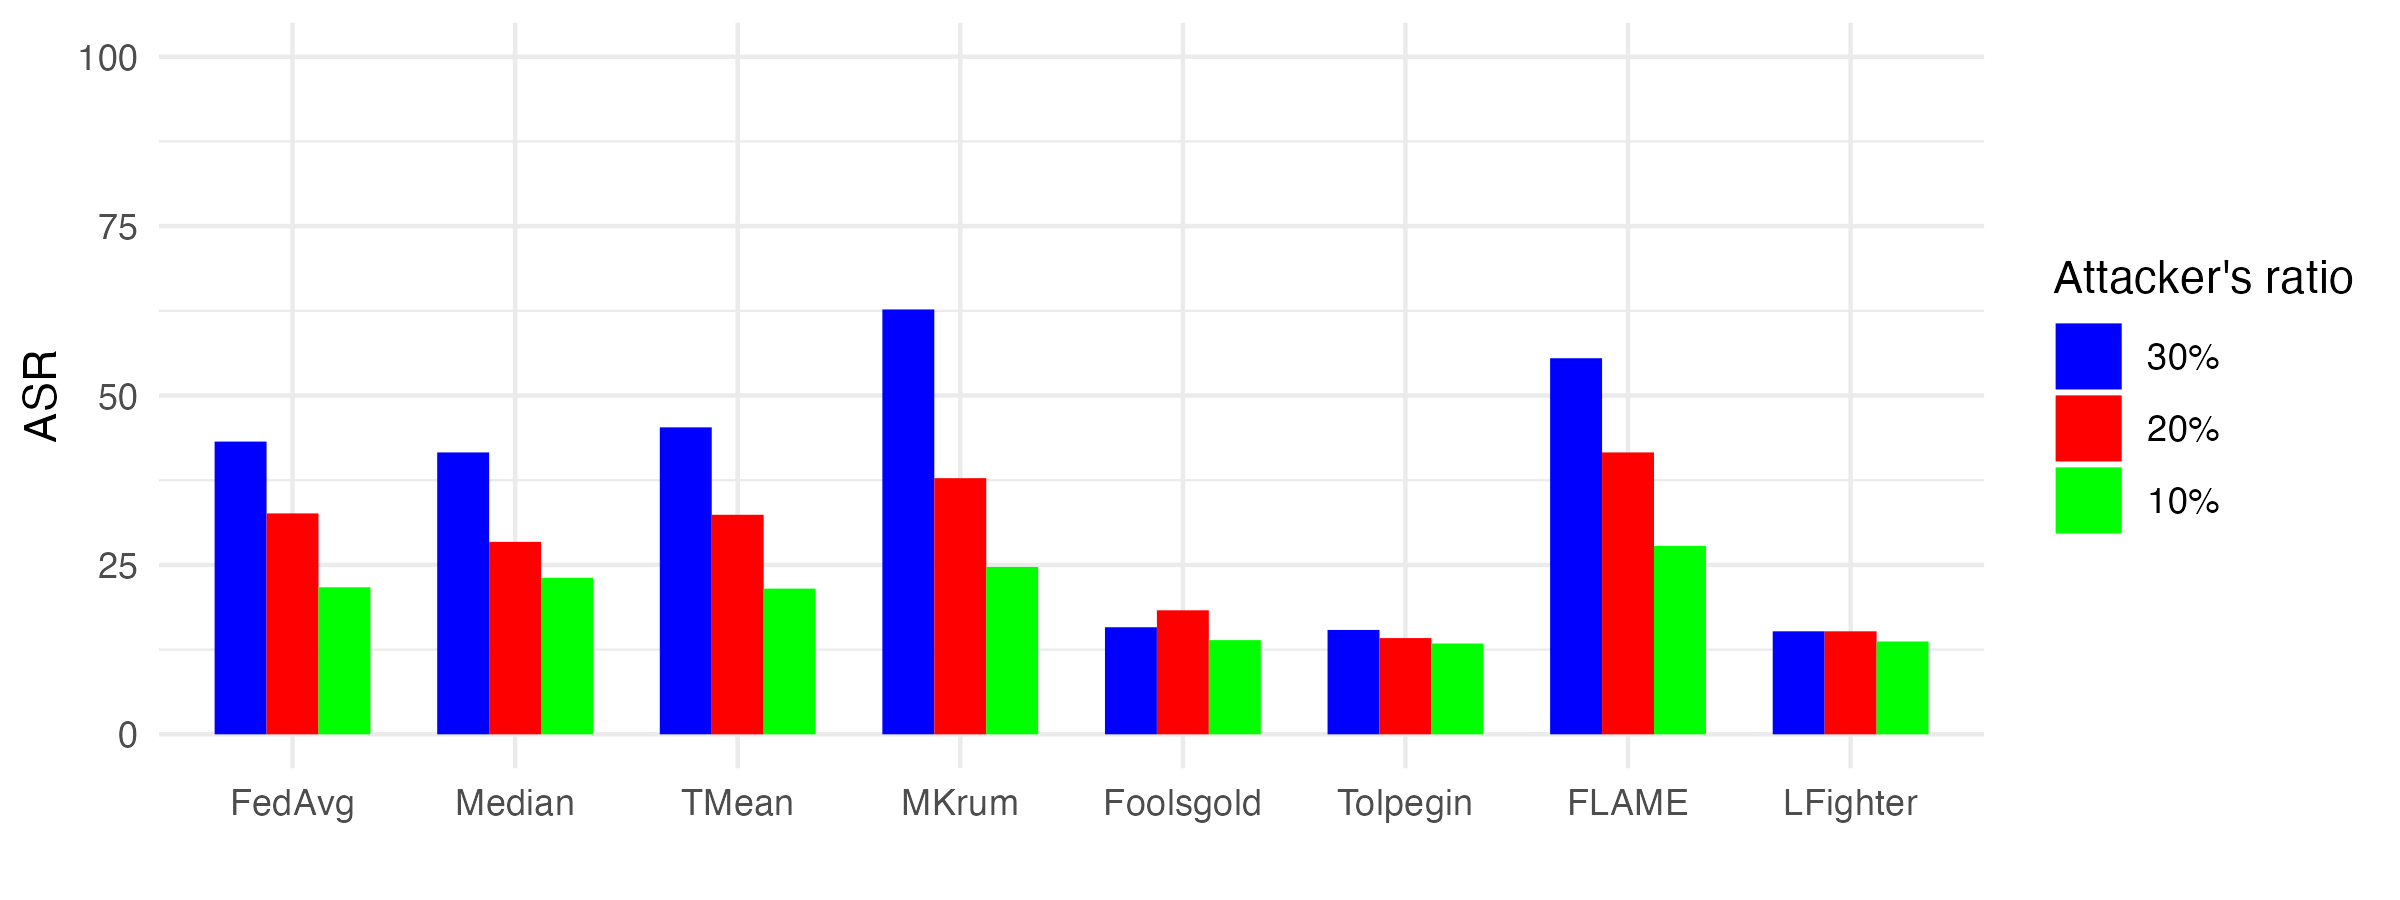
\includegraphics[scale=0.88]{ASR_std.png}
    \caption{ASR for standard label flipping}
    \label{fig:ASR_std}
\end{figure}

\begin{figure}[h!]
    \centering
    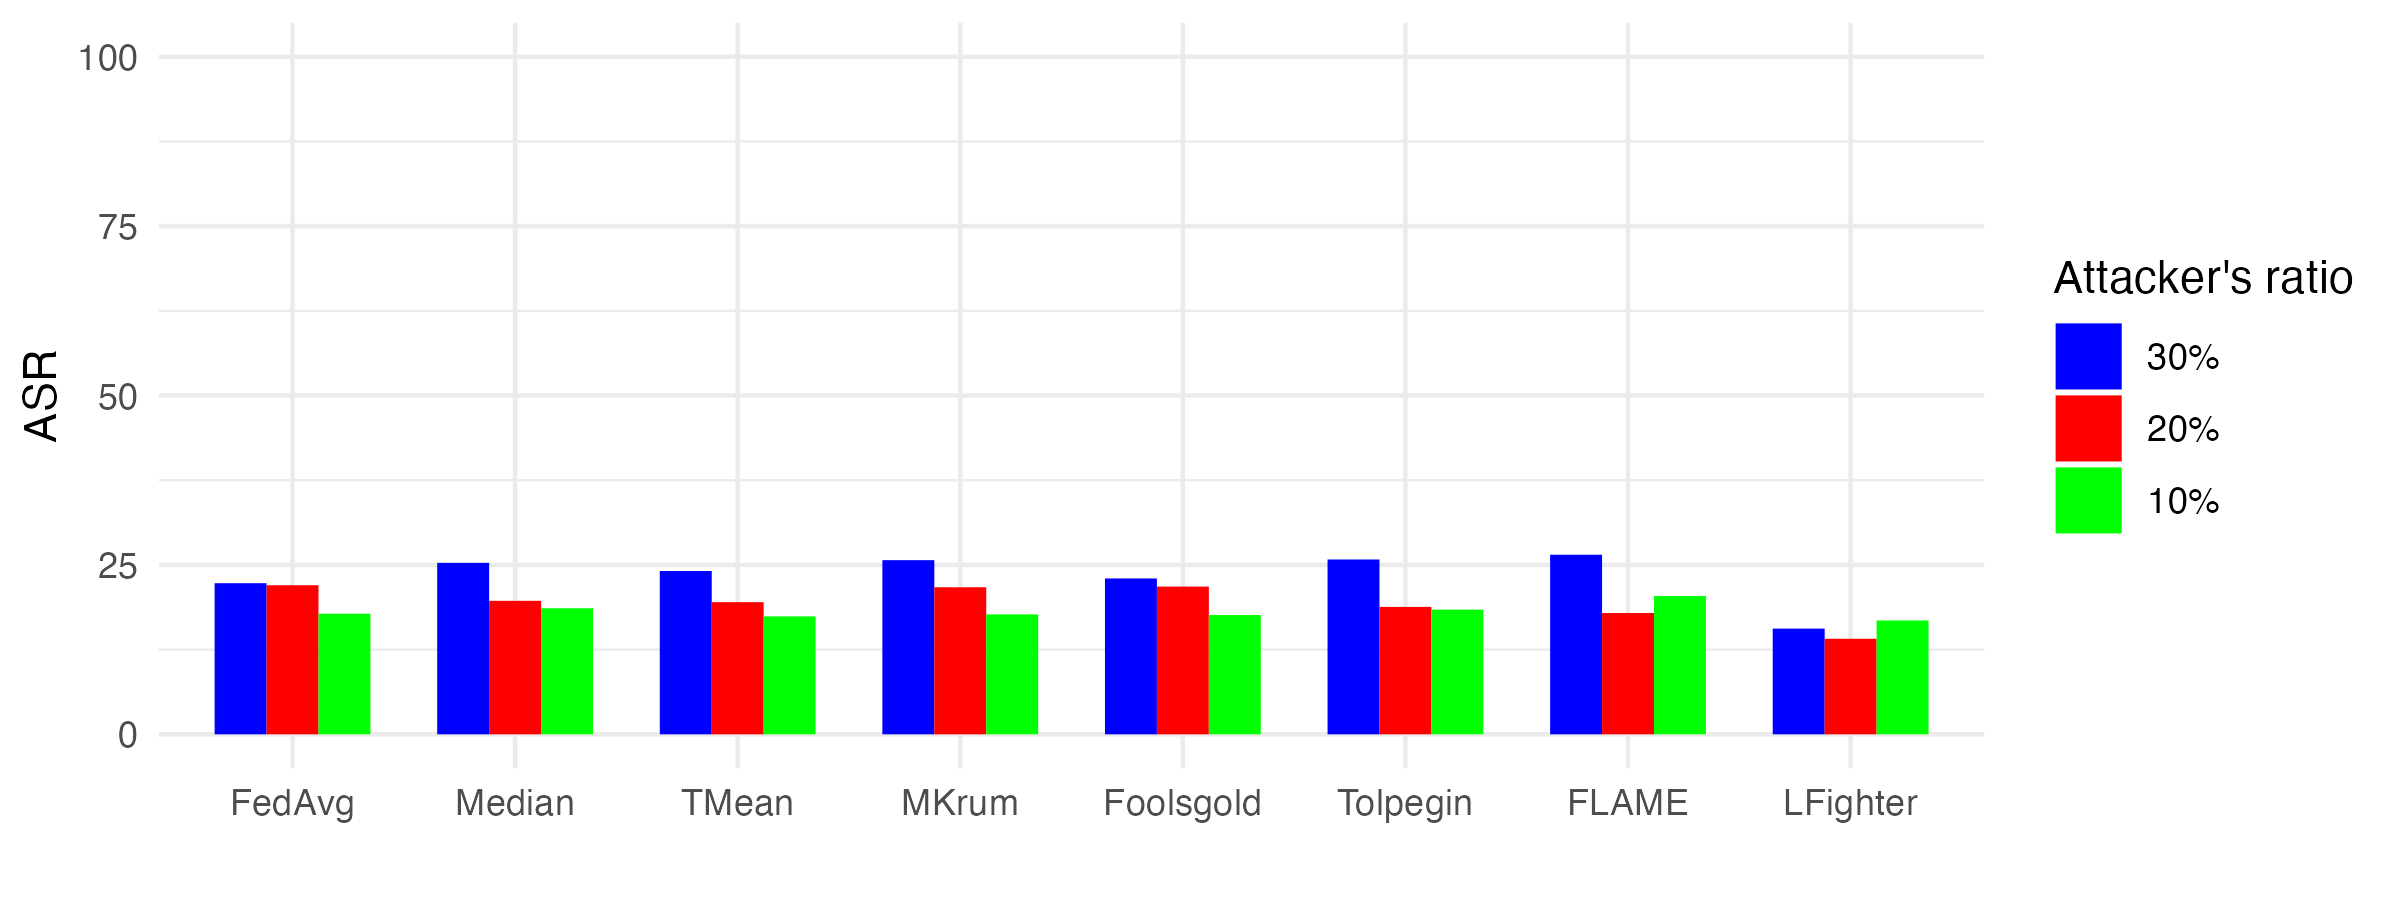
\includegraphics[scale=0.88]{ASR_ent.png}
    \caption{ASR for Entropy-based label flipping}
    \label{fig:ASR_ent}
\end{figure}

\begin{figure}[h!]
    \centering
    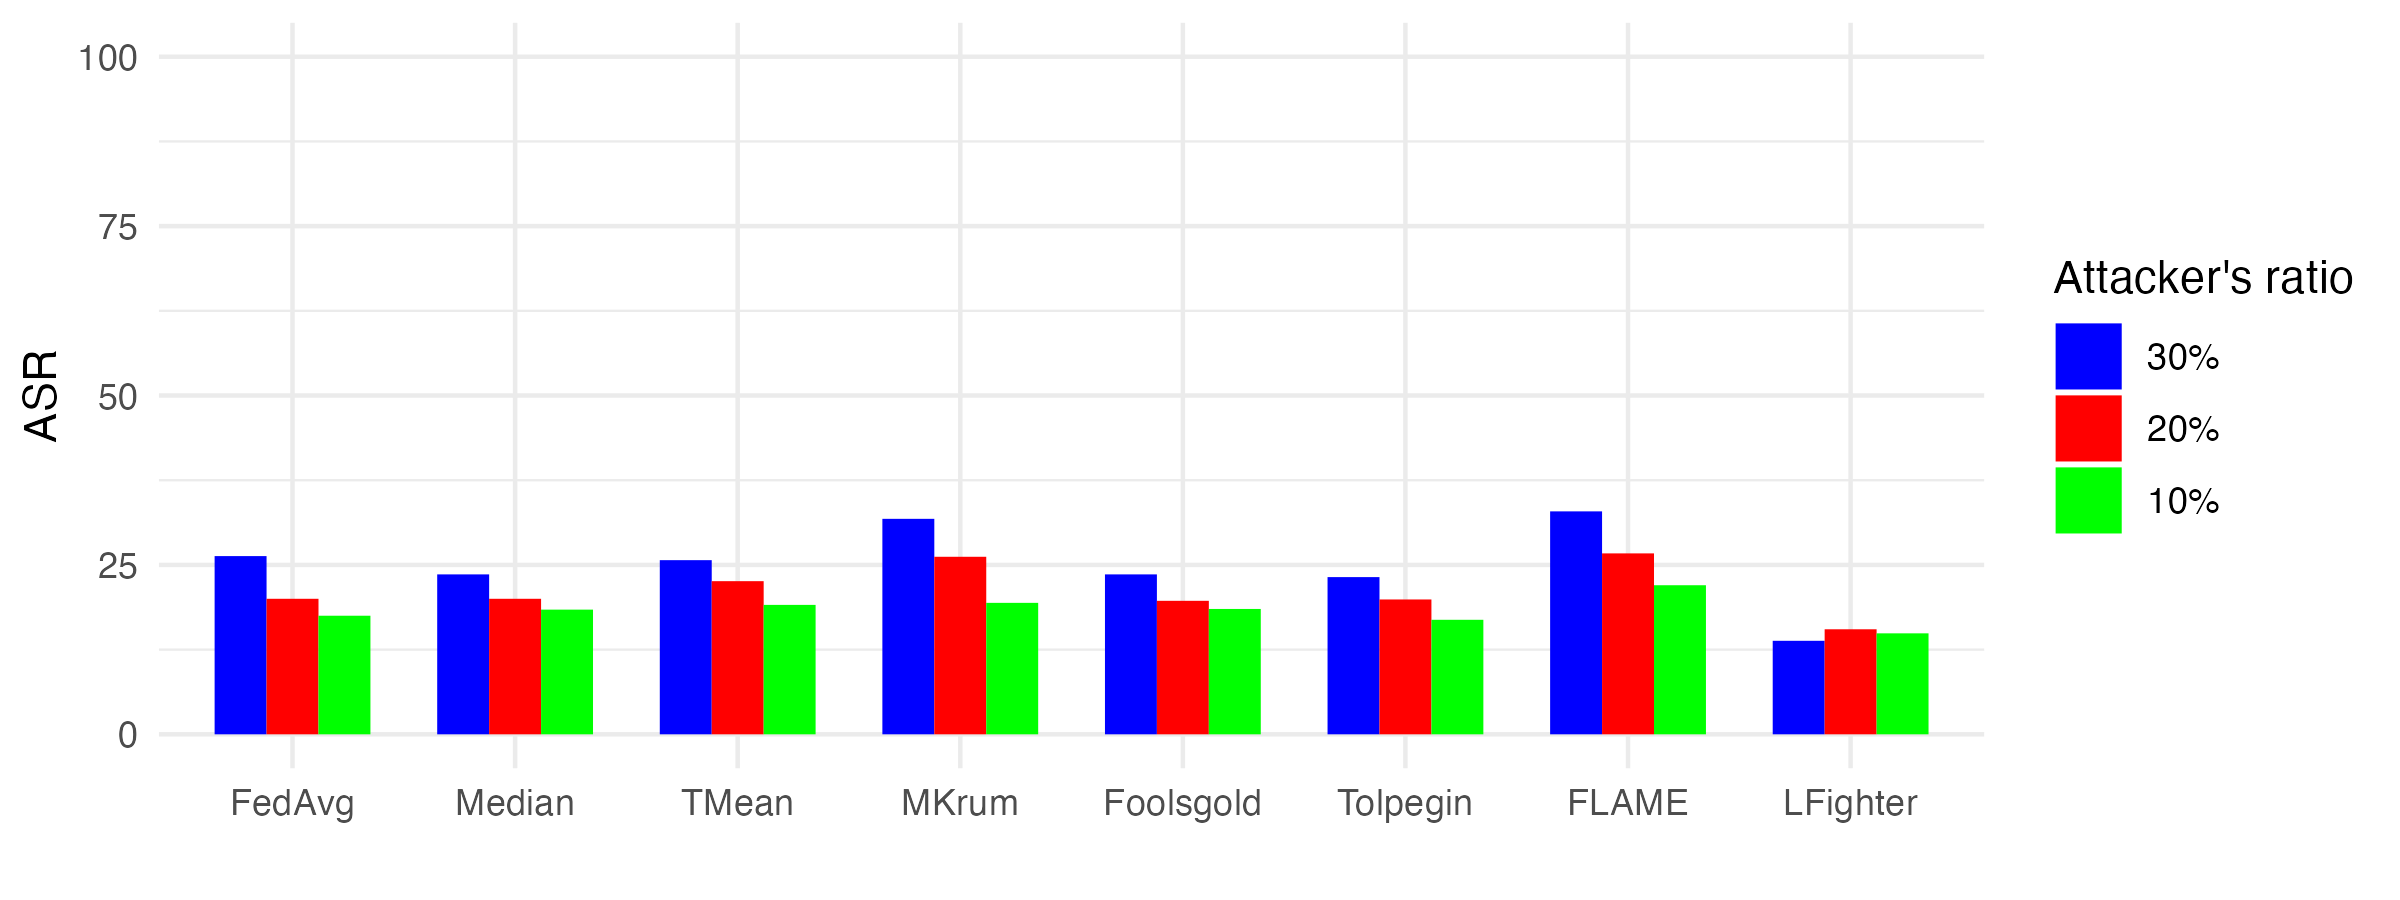
\includegraphics[scale=0.88]{ASR_clos.png}
    \caption{ASR for Closeness-based label flipping}
    \label{fig:ASR_clos}
\end{figure}
 
\pagebreak
